\clearpage
\section{RE intercepts plus catch-up, lambda fixed at Barro 0.98}
2026-09-17 SA panel, full sample: log real GDP per worker. 74 countries, 8670 observations, 1950-Q1--2026-Q2. Fitted countries: 74. Observations: 8670. Log-likelihood: 23563.79. Ergodic mean of the cycle $E[z]=0.0601$ (0.0275).
Permanent RE intercepts and catch-up $y_{it}=a_i + g t + b_i\lambda^{t-T_{i0}}+z_{it}$ with $\alpha=-5.7753$ (0.0388), $\omega=0.6254$ (0.0064), $\lambda=0.9800$ (fixed), $\omega_b=0.4180$ (0.0097). Posterior-mean $a_i$: mean -5.787, min -8.120, max -4.292. Posterior-mean $b_i$: mean -0.014, min -0.977, max 0.989. Common slope $g=0.0117$ (0.0005).
\begin{table}[h]
\centering
\caption{Regime AR(1), transition matrix, and ergodic $\pi$. Columns are regimes.}
\begin{tabular}{lccc}
\toprule
 & (0) & (1) & (2) \\
\midrule
$\mu$ & -0.9844 & 0.0000 & 0.3062 \\
 & (0.1493) & --- & (0.0292) \\ \addlinespace
$\sigma$ & 0.0760 & 0.0187 & 0.0069 \\
 & (0.0028) & (0.0005) & (0.0001) \\ \addlinespace
$\rho$ & 0.9899 & 0.9900 & 0.9898 \\
 & (0.0007) & (0.0001) & (0.0008) \\ \addlinespace
$\Pi_{0\cdot}$ & 0.6929 & 0.2871 & 0.0199 \\
 & (0.0328) & (0.0332) & (0.0091) \\ \addlinespace
$\Pi_{1\cdot}$ & 0.0543 & 0.8882 & 0.0575 \\
 & (0.0067) & (0.0095) & (0.0066) \\ \addlinespace
$\Pi_{2\cdot}$ & 0.0091 & 0.0455 & 0.9454 \\
 & (0.0026) & (0.0057) & (0.0052) \\ \addlinespace
$\pi$ & 0.0899 & 0.4275 & 0.4826 \\
 & (0.0095) & (0.0214) & (0.0248) \\ \addlinespace
\bottomrule
\end{tabular}
\end{table}
\begin{figure}[h]
\centering
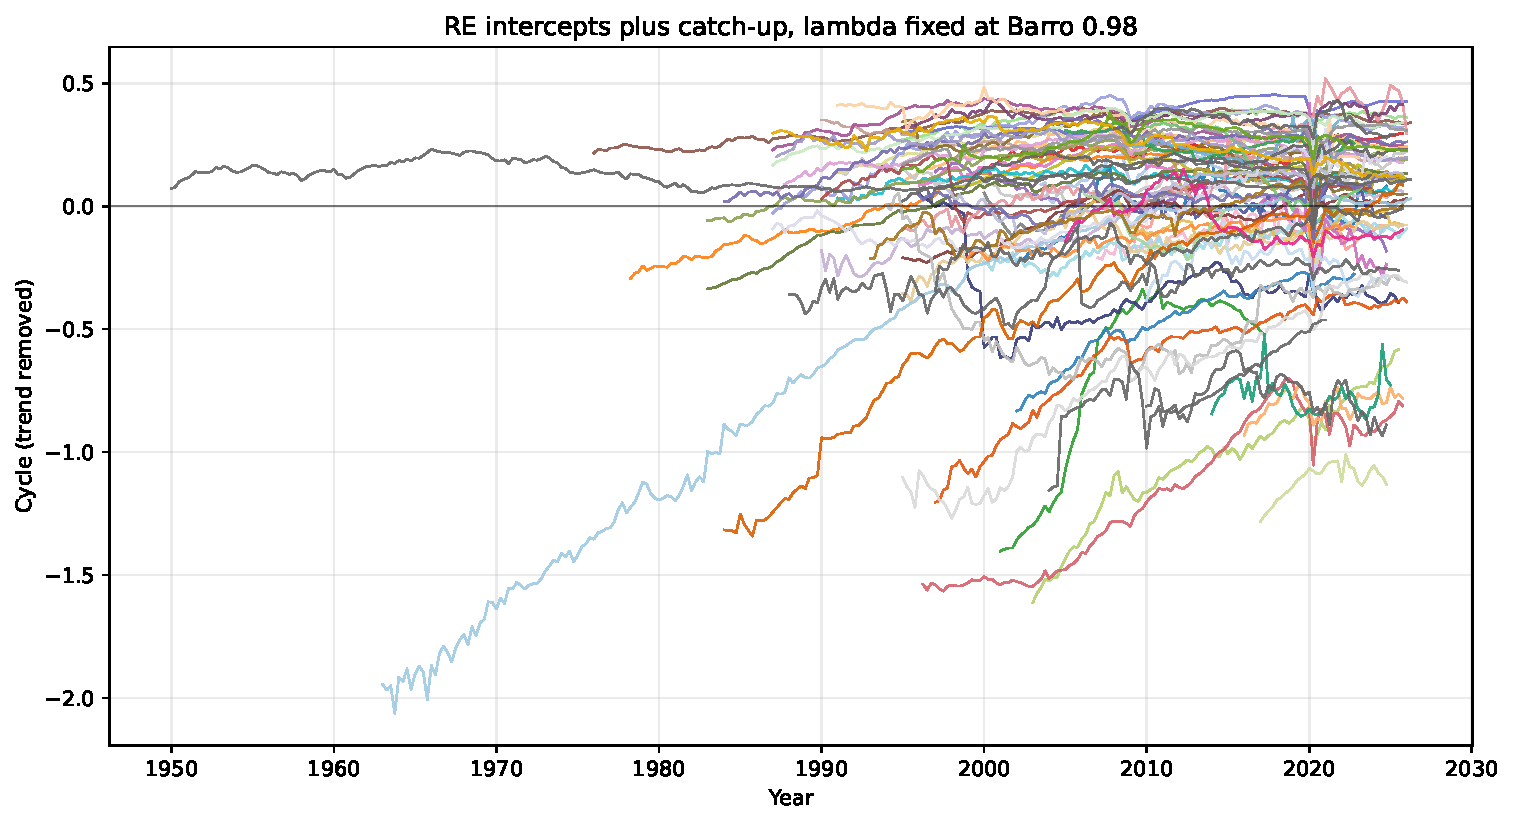
\includegraphics[width=0.75\textwidth]{figs/cycle_lambda_barro.pdf}
\caption{Country cycles after removing $a_i + g t + b_i\lambda^{t-T_{i0}}$ (posterior-mean $a_i$, $b_i$).}
\end{figure}
